\chapter[Do countries compete over corporate tax rates?]{Countries do compete \\over corporate tax rates}
\vspace{-11pt}
The continuous reduction of the corporate income tax burden may seem to some to be detrimental to government tax revenues. Actually, lowering firm income tax rates is part of a strategic game in which countries have found themselves not to lose existing and potential capital after the surge of internationalization and trade. \textcite{dev-loc-red-08}, in their paper titled "Do countries compete over corporate tax rates?", model this interaction between states as a competitive game. First, by constructing Nash equilibrium tax rates and then comparing them with actual tax rates, they explain the decline in corporate income tax rates with the progressive loosening of capital controls.
\vspace{-7pt}
\section{A theoretical framework}
\vspace{-10pt}
\subsection{A model of corporate tax competition}
In a tax-competitive setting with two countries, home and foreign, both have inhabitants and a multinational firm with its headquarters. Every resident benefits from consuming a private good, \(x\), and of a public good, $g$. The provision of the public good by the local government is financed through a source-based corporate tax on the profits realised in the country. Consequently, the global after-tax profit of the multinational with the parent in the home country is:
\begin{align}
\Pi&=\overbrace{f(k)-rk-q-\tau(f(k)-ark-q)}^{\textsubscript{home profit}}+\overbrace{(1-\tau^*)(q-c)}^{\textsubscript{foreign profit}}\\
&=(1-\tau)(f(k)-zrk-q)+(1-\tau^*)(q-c)\notag
\end{align}
where the home profit is realised from the output, $f(k)$, employing $k$ units of capital, which is purchased from households at price $r$, and a discrete input bought from the affiliate in the foreign country at price $q$, i.e. the transfer price. In the home country, the firm pays the tax  $\tau(f(k)-ark-q)$, where $0\le\tau\le1$ is the statutory tax rate, and $a\ge0$ is the portion of the cost of capital deductible from revenues, i.e. the rate of allowance. Finally, the profit of the foreign affiliate, $q-c$, where $c$ is the cost of producing the discrete input, is taxed at the foreign statutory tax rate $\tau^*$.

In their model, \textcite{zo-mi-86} consider the presence of only one instrument at the government's disposal, a tax on returns to capital, here, \textcite{dev-loc-red-08} provide the government with the possibility to set $a$, and consequently influencing the EMTR, that is $z-1=\frac{(1-a\tau)}{1-\tau}-1$.
\vspace{-6pt}
\subsection{The players' perspective}
%The objective of both parent firms is to maximize the global profits, $\Pi$ and $\Pi^*$, having as control variables the transfer prices, $q$ and $q^*$, and the capital, $k$ and $k^*$, resulting, for the home multinational, in $\max\limits_{q, k} \Pi$. In doing so, firms consider the possibility of being convicted of a fine by the government if they disobey the arm's length principle for transfer pricing. Namely, a fine proportional to the reduced tax base is levied: $EF=\alpha(q-c)^2$, where $(q-c)$ is the reduction in the tax base, and $\alpha$  a coefficient determining the extent of the fine. The maximization problem of the home multinational breaks down as follow, and it illustrates how the multinational firm chooses where to locate investments and corporate income:
The objective of both parent firms is to maximize the global profits, $\Pi$ and $\Pi^*$, having as control variables the transfer prices, $q$ and $q^*$, and the capital, $k$ and $k^*$, resulting, for the home multinational, in $\max\limits_{q, k} \Pi$. In doing so, firms consider the possibility of being convicted of a fine $EF$ by the government if they disobey the arm's length principle for transfer pricing. Therefore, the maximization problem of the home multinational breaks down as follow, and it illustrates how the multinational firm chooses where to locate investments and corporate income:
\begin{align}\label{eq2.3}
        \scalemath{0.9}{\max\limits_{q, k}\Pi-EF \quad \Longrightarrow \quad (i)\, \frac{\partial \Pi}{\partial q}=0\, , \, q=c+\frac{\tau-\tau^*}{2\alpha}\quad ; \quad (ii)\, \frac{\partial \Pi}{\partial k}=0\, , \, f'(k)=zr}
\end{align}
%\begin{align}
%        &\max\limits_{q, k}\Pi=(1-\tau)(f(k)-zrk-q)+(1-\tau^*)(q-c)-\underbrace{\alpha(q-c)^2}_{\textsuperscript{EF}}\\
%        &\label{eq2.3}(i)\, \frac{\partial \Pi}{\partial q}=0\; \rightarrow \; q=c+\frac{\tau-\tau^*}{2\alpha}\quad ; \quad (ii)\, \frac{\partial \Pi}{\partial k}=0\; \rightarrow \; f'(k)=zr
%\end{align}
From Eq. \ref{eq2.3} (i), it follows that $q$ is the profit-maximizing transfer price, and it depends on the difference between the two statutory rates. As $\tau$ increases, the home parent is more encouraged to rise $q$ in order to shift the profits to the foreign affiliate, where the statutory tax rate is lower, and conversely, if $\tau^*$ grows. In Eq. \ref{eq2.3} (ii), the capital is implicitly defined and depends on the interest rate $r$ and on $z$. A higher $z$ requires a higher capital productivity $f'(k)$, which is associated with a lower capital stock $k$ in the country.

%Moreover, from Eq. \ref{eq2.3} (ii), the global demand for capital can be derived as $k(zr)+k(z^*r)=2\kappa$, which states that the sum of demands for capital by the home and foreign multinational is equal to the global supply of capital.

Once described the general setting and the firm's perspective, it is now necessary to analyze the country's behaviour in the strategic tax game, with the ultimate goal of finding its symmetric Nash equilibrium and reaction functions. In other words, how and if a government reacts when other countries change their tax rates.

The home government maximizes the welfare in the country by choosing its own statutory tax rate $\tau$ and the coefficient $z$, taking the foreign rates, $\tau^*$ and $z^*$, as given: $\max\limits_{\tau,z}W=r\kappa+\Pi-EF+v(g)$. As the inhabitants fully own the firm, the first three terms represent the income of the residents, consisting of the return from the capital $\kappa$ borrowed to the firm, the profit $\Pi$ minus the possible fines $EF$, and $v(g)$, the utility from the consumption of the public good.

%In order to provide the public good $g$ to households, the government collects taxes on corporate income and levies fines. For simplicity, the latter is fully consumed by the administrative costs of collection, and therefore, the budget constraint of the government reads, where $\pi(zr)$ is the profit function, as: $g=\tau(\pi(zr)-q)+(z-1)rk(zr)+\tau(q^*-c)$. The first two terms are the tax collected by the home government from the national parent as a mixture of the statutory tax base and the EMTR base. The last term represents the revenues from the profits realised by the local affiliate of the foreign parent.

The budget constraint of the government, where $\pi(zr)$ is the profit function, is $g=\tau(\pi(zr)-q)+(z-1)rk(zr)+\tau(q^*-c)$. The first two terms are the tax collected by the home government from the national parent as a mixture of the statutory tax base and the EMTR base. The last term represents the revenues from the profits realised by the local affiliate of the foreign parent.

The government maximizes $W$, subject to its budget constraint, and the optimal tax rates result from the first-order conditions: $\frac{\partial W}{\partial \tau}=W_\tau=0$ and $\frac{\partial W}{\partial z}=W_z=0$. In equilibrium, it is now imposed that both countries choose the same rates, ($\tau$, $z$)=($\tau^*$,$z^*$). In other words, a symmetric Nash equilibrium of the governments' choices (strategies) is reached. Solving the optimization problem of the government at the symmetric Nash equilibrium, i.e. ($\tau=\tau^*=\hat{\tau}, z=z^*=\hat{z}$), $\hat{\tau}$ and $\hat{z}$ result in:
\begin{align}
    \label{eq2.4}&W_\tau=\frac{\partial \hat{\Pi}}{\partial \tau}+v'\frac{\partial g}{\partial \tau}\quad \xrightarrow{\text{solving for }\hat{\tau}} \quad \hat{\tau}=\frac{\alpha(v'-1)(\pi-c)}{v'}\\[3pt]
\label{eq2.5}
&\scalemath{0.91}{W_z=\frac{\partial \hat{\Pi}}{\partial z}+v'\frac{\partial g}{\partial z}+\frac{\partial W}{\partial r}\frac{\partial r}{\partial z}\; \xrightarrow{\text{solving for }\hat{z}} \; \frac{\hat{z}-1}{\hat{z}}=\frac{(v'-1)(1-\hat{\tau})}{v'\epsilon}+\frac{\partial W}{\partial r}\left( \frac{z\partial r}{r\partial z}\right) \frac{1}{v'k\epsilon}}
\end{align}
Eq. \ref{eq2.4} characterizes $\hat{\tau}$, the statutory tax rate in equilibrium. It depends on the statutory tax base ($\pi-c$), and it is inversely proportional to the sensitivity of the tax base to the statutory tax, $\left(\frac{1}{\alpha}\right)$ from Eq. \ref{eq2.3} (i). This suggests that as the tax base becomes more sensitive to changes in the statutory tax rate (higher $\frac{1}{\alpha}$), the equilibrium tax rate decreases. Eq. \ref{eq2.5} defines the optimal EMTR, ($\hat{z}-1$). Interestingly, if the government aims to increase its revenue, and the elasticity of taxable income $\epsilon$ is inversely related to the EMTR, then a higher value of $\epsilon$ would result in a lower EMTR. This relationship suggests that when firms are more responsive to changes in tax rates (higher $\epsilon$), the government needs to set a lower EMTR to generate the desired level of revenue.
\vspace{-7pt}
\subsection{Reaction functions} \label{reaction_functions}
Theoretically, both the tax instruments of a government, $\tau$ and $z$, react to both $\tau^*$ and $z^*$, their reaction functions are $\tau=T(\tau^*,z^*)$, $z=Z(\tau^*,z^*)$. The best approximation around the Nash equilibrium of the reaction functions can be obtained by linearizing $W_\tau$ and $W_z$ using total differentiation.
\begin{equation}\label{eq2.6}
\scalemath{0.90}{\left(
\begin{matrix}
W_{\tau\tau} & W_{\tau z} \\
W_{\tau z} & W_{zz}
\end{matrix}
\right)
\left(
\begin{matrix}
\partial \tau \\
\partial z
\end{matrix}
\right)=-
\left(
\begin{matrix}
W_{\tau\tau^*} & W_{\tau z^*} \\
W_{z \tau^*} & W_{zz^*}
\end{matrix}
\right)
\left(
\begin{matrix}
\partial \tau^* \\
\partial z^*
\end{matrix}
\right)}
\end{equation}
From Eq. \ref{eq2.6}, it is now possible to describe the slopes of the reaction functions. Firstly, $\tau$ and $\tau^*$ are strategic complements, $W_{\tau\tau^*}>0$. If $\tau^*$ grows, $q$ decreases and the statutory tax base $\pi-c$ increases, resulting in a higher $\tau$. Secondly, $\tau$ and $z^*$ are strategic complements, $W_{\tau z^*}>0$. If $z^*$ grows, results in a lower price of capital and higher profits $\pi(zr)$ and higher $\tau$. Moreover, $z$ and $\tau^*$ are strategically independent, $W_{z\tau^*}=0$. If $\tau^*$ grows, this influences the transfer prices $q$ and $q^*$, but it does not influence $z$. Lastly, \textcite{dev-loc-red-08} finds that $z$ and $z^*$ are also strategic complements, $W_{z z^*}>0$, but only imposing further assumptions.

In conclusion, the key findings of the theoretical model built by  the authors are the following. First, there are positive effects within the same tax, i.e. $\frac{\partial \tau}{\partial \tau^*}>0$, $\frac{\partial z}{\partial z^*}>0$. Second, between different taxes, the effects are smaller, in particular $\frac{\partial z}{\partial \tau^*}<0$, $\frac{\partial \tau}{\partial z^*}>0$.
\vspace{-10pt}
\section{Testing the theory}
\vspace{-10pt}
\subsection{Equations for the reaction functions}\label{empirical-spec}

Once found the theoretical assumptions to test, \textcite{dev-loc-red-08} expresses, and expands, the empirical formulation for both the reaction functions, $T(\cdot)$ and $Z(\cdot)$. At first, in both reaction functions, a vector $\textbf{X}$ of variables that affect public spending is included. Considering $n$ countries, the country's $i$ reaction functions are ${\tau}_i=T_i(\boldsymbol{\tau}_{-i},\textbf{z}_{-i},\textbf{X}_i)$ and $z_i=Z_i(\boldsymbol{\tau}_{-i},\textbf{z}_{-i},\textbf{X}_i)$. A linear approximation of both at the Nash equilibrium, like in Section \ref{reaction_functions}, is:
\begin{align}
\vspace{-5pt}
\label{eq2.7} \scalemath{0.9}{\tau_{i,t}=\hat{\tau_i}+\sum_{j\neq i}\frac{\partial T_i}{\partial \tau_j}\boldsymbol{\tau}_j+\sum_{j\neq i}\frac{\partial T_i}{\partial z_j}\textbf{z}_j+\boldsymbol{\eta}_{1}'\textbf{X}_i \quad \quad \quad i=1,\dots,n}\\
\label{eq2.8} \scalemath{0.9}{z_{i,t}=\hat{z_i}+\sum_{j\neq i}\frac{\partial Z_i}{\partial \tau_j}\boldsymbol{\tau}_j+\sum_{j\neq i}\frac{\partial Z_i}{\partial z_j}\textbf{z}_j+\boldsymbol{\eta}_{2}'\textbf{X}_i \quad \quad \quad i=1,\dots,n}
\vspace{-5pt}
\end{align}
where $\hat{\tau_i}$ and $\hat{z_i}$ are the Nash equilibrium rates, and $\boldsymbol{\eta}_{1}'$ and $\boldsymbol{\eta}_{2}'$ are the coefficients for $\textbf{X}_i$. The second and third terms describe the behaviour of the reaction functions to changes in the rates of the other countries. Clearly, this impacts the calculations significantly and, therefore, \textcite{dev-loc-red-08} replaces them like follows, e.g. $\frac{\partial T_i}{\partial \tau_j}=\beta_1\omega_{ij}$ and $\frac{\partial T_i}{\partial z_j}=\gamma_1\omega_{ij}$, assuming every country exhibits a uniform response to the weighted average tax rates of the other countries, $\overline{\tau}_i$ and $\overline{z}_i$.

To conclude, the following are the equations used by the authors to empirically test the theoretical assumptions of the reaction functions modelled in the previous sections:
\vspace{-5pt}
\begin{align}
&\label{eq2.9} \scalemath{0.9}
{\tau_{i,t}=\beta_1\overline{\tau}_{i,t}+\gamma_1\overline{z}_{i,t}+\boldsymbol{\eta}_{1}'\textbf{X}_{it}+\phi_{1i}+T_{1it}+\varepsilon_{1it} \quad \quad i=1,\dots,n}\\
&\label{eq2.10} \scalemath{0.9}{z_{i,t}=\beta_2\overline{\tau}_{i,t}+\gamma_2\overline{z}_{i,t}+\boldsymbol{\eta}_{2}'\textbf{X}_{it}+\phi_{2i}+T_{2it}+\varepsilon_{2it} \quad \quad i=1,\dots,n}
\vspace{-5pt}
\end{align}
where $\phi_{1i}$, $\phi_{2i}$ are country-specific fixed effects, and $T_{1it}$, $T_{2it}$ are country-specific time trends, both included to account for potential unobserved factors.
\vspace{-7pt}
\subsection{Data}\label{dev-data}

To run their empirical model, \textcite{dev-loc-red-08} use panel data for 21 OECD countries between 1982 and 1999.

\begin{figure}[h]
    \centering
    \captionsetup{font=footnotesize}\caption{time series for avg. statutory tax rate and tax wedge, \textcite{dev-loc-red-08}}
    \label{dev-rate-fall}
    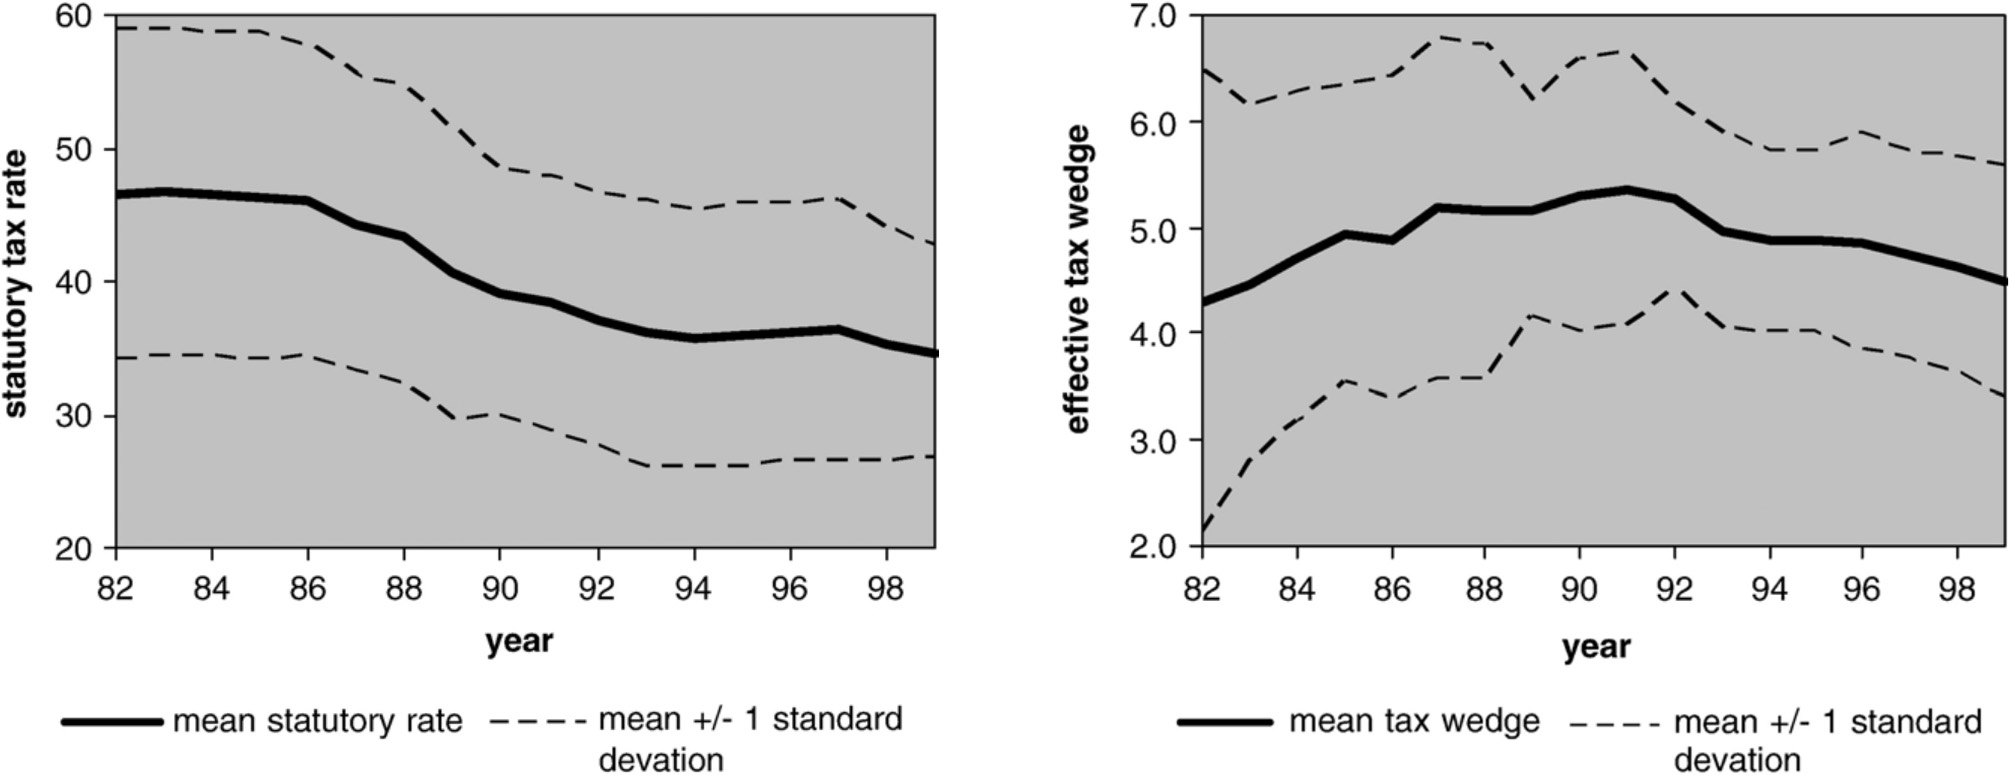
\includegraphics[width=0.74\textwidth]{img/devereux-rates.jpg}
    \vspace{-5pt}
\end{figure}
First of all, the authors use the uniform weighted mean of the statutory tax rates, revised for the local statutory rates, in the 21 countries. Next, the EMTR, which typically is ambiguous to measure and, from Eq. \ref{eq2.3} (ii), is $z-1= \frac{f'(k)-r}{r}$. Here the authors decide to refer to it as $f'(k)-r$, the difference between the marginal product of capital and the interest rate, i.e. the tax wedge. The time series of both these measures are shown in Fig. \ref{dev-rate-fall}. On the left of Fig. \ref{dev-rate-fall}, it can be clearly seen how the mean statutory tax rate in the 21 OECD countries fell from nearly 50\% in 1982 to close to 35\% in 1999. On the other hand, the mean tax wedge, over the same period, slightly increased and reduced its standard deviation. In addition to these two measures, a number of control variables are included to explain better how countries set their rates.

%Lastly, in addition to the country-specific fixed effect and time trends factors, $\textbf{X}$ consists of the following control variables: the highest marginal income tax rate, since the corporate tax rate is usually evaluated as a "backstop" for personal income, the revenue need of the government, its openness and size, dummies about the political orientation, and some demographic variables.
\vspace{-5pt}
\subsection{Econometric issues}

Before presenting the regression results, the endogeneity of $\overline{\tau}_{i,t}$ and $\overline{z}_{i,t}$ in Eq. \ref{eq2.9} and \ref{eq2.10}, needs to be tackled and here, the authors implement an instrumental variable approach.

The chosen instruments are the weighted means of the control variables in other countries, e.g. $\overline{\tau}_{i,t}=\sum_{j\neq i}\omega_{ij}\tau_{jt}$. Weights related either to the size of the other countries (measured in GDP units) or to FDI flows are shown to be endogenous by \textcite{dev-loc-red-08}. Therefore, in the Section below, only the results based on uniform weights are displayed. To sum up, using as instrumental variables the (uniform) weighted average of the controls leads to an $R^2$, in the first stage regression, between $0.87$ and $0.99$ for both rates, confirming the validity of the instruments.
\vspace{-10pt}
\section{Empirical results}
\vspace{-10pt}
\subsection{Regression results}
\vspace{-5pt}
\begin{table}[!h]
\parbox{.53\linewidth}{
\centering
\captionsetup{font=footnotesize,justification=centering}\caption{regression results,\\ 
\textcite{dev-loc-red-08}\label{tab:dev-regr}}
\scalebox{0.65}{
\begin{tabular}{lp{3.8cm}p{3.8cm}}
\hline
                                     & \textbf{Statutory rate}, $\tau_{it}$ & \textbf{Eff. tax wedge}, $w_{it}$ \\ \hline
$\overline{\tau}_{it}$                                 & 0.678          & -0.012             \\
                                     & (2.5)           & (0.19)               \\
$\overline{w}_{it}$                                 & -1.362        & 0.766               \\
                                     & (1.04)          & (2.35)               \\
Income tax rate                      & 0.16           & 0.007               \\
                                     & (2.95)          & (0.84)               \\
Size                                 & 0.54           & -0.02              \\
                                     & (2.55)          & (0.22)               \\
Public cons./GDP               & 0.007           & 0.07              \\
                                     & (0.03)          & (0.99)               \\                                     
Observations                         & 378            & 378                 \\
R-squared                            & 0.93           & 0.77                \\ \hline
\end{tabular}}}
\hfill
\parbox{.47\linewidth}{
\centering
\captionsetup{font=footnotesize,justification=centering}\caption{comparison between hypothetical Nash eq. rates with fixed capital controls and actual ones, \textcite{dev-loc-red-08}}
\scalebox{0.57}{
\begin{tabular}{lllll}
\hline
Control variable data                        & 1983    & 1997    & 1997    & 1983    \\
Capital control data                         & 1983    & 1997    & 1983    & 1997    \\
Actual average tax rates                     & 46.60\% & 36.30\% & n.a.    & n.a.    \\
Nash eq. avg. stat. tax rates & 44.20\% & 35.80\% & 44.50\% & 36.70\% \\ \hline
\end{tabular}}}
\end{table}

In Table \ref{tab:dev-regr}, the estimated coefficients resulting from the regression are reported, together with the $t$-statistics. Starting from the statutory rate, $\tau_{it}$, the main effects come from $\overline{\tau}_{it}$, the income tax rate and the size. As backed by similar results in the literature, e.g. \textcite{slemrod}, the corporate income statutory tax rate plays a key role as "backstop" for individual income tax. The lack of a corporate income tax rate would encourage individuals to "incorporate" (shift) their personal income, to avoid the tax. Here, the presence in the country of a higher top-income tax has a positive effect on $\tau_{it}$, however, it has no effect on the tax wedge. Likely, the country's size leads to a higher $\tau_{it}$, confirming the general view in the literature that smaller countries levy lower tax rates. Nevertheless, the biggest correlation comes from the uniform weighted average tax rate of the other countries, $\overline{\tau}_{it}$, with a coefficient of $0.678$. On the tax wedge's side, only the average of the other countries' tax wedge has a (positive) significant effect on country $i$, $w_{it}$ stops at $0.766$.

The main two assumptions derived from the theoretical model are reflected in the results. First, the "own-tax" effects are positive, i.e. $\frac{\partial \tau}{\partial \tau^*}>0$, $\frac{\partial z}{\partial z^*}>0$, because both reactions are mainly correlated with the other countries' choices with respect to the same rate. Second, the "cross-tax" effects are smaller, however, this result is not rock solid and depends on the weight used.

\vspace{-5pt}
\subsection{Can the model explain the evolution of taxes over time?}

The results in Table \ref{tab:dev-regr} reveal an interaction over statutory tax rates and effective tax wedges between countries, however, the authors further investigate, excluding it, another possible source of variation in taxation levels. Does yardstick competition, as suggested by \textcite{besley}, also play a role in the strategic interaction between countries? They further expand Eq. \ref{eq2.9} and \ref{eq2.10} allowing country $i$ to react differently to other countries' rates whether there are strong capital controls between the two or not. \textcite{dev-loc-red-08} find clear evidence that between countries without capital controls in place, the competition over statutory tax rates is stronger. More simply, the lack of capital controls between two countries, and consequently larger (and freer) capital flows, triggers competition (over the statutory rate) between countries to attract corporate profits. On the other hand, capital controls do not appear to be particularly significant for the interaction over effective tax wedges.

\textcite{dev-loc-red-08} conclude their analysis with one last striking result. To further emphasize the role of capital controls in causing tax competition, which ultimately results in lower statutory tax rates, they compare the actual average tax rates with hypothetical Nash equilibrium ones built fixing the capital control levels. In other words, they build an hypothetical statutory tax rate for 1997 keeping the capital controls in place in 1983, and conversely. The outcomes confirm the impact of capital controls on tax rates: if in 1997 there had been the capital control of 1983, the equilibrium statutory rate would likely have remained high, $44.5\%$. Vice versa, in 1983, with the (more relaxed) capital controls of 1997, the equilibrium statutory rate would probably have been $36.7\%$.

Overall, the model and the results suggest that governments of more open jurisdictions strategically interact over tax rates with the intent of not losing capital inflows. Non-participation would incentives firms to relocate their assets. It is therefore credible to think that they will continue this competition, preventing the harmful effects of a "race to the bottom" while offsetting with broader tax bases and strengthening international tax coordination efforts. This is the background to the OECD's BEPS plan, discussed~below.
